\chapter{Elméleti megalapozás}\label{chapter1}

\section{Piacelemzés}

A dolgozat ezen részében megvizsgáljuk a konténerizációs világ adta
lehetőségeket, és bemutatjuk a Zebrafish által kitöltött piaci rést. A
felhőplatformokra való nagyfokú összpontosítás miatt a konténerizáció világa az
elmúlt években jelentős növekedésnek indult, mivel a vállalatok egyre inkább
felismerik a konténerek előnyeit: a hordozhatóságot, a skálázhatóságot és az
erőforrás-hatékonyságot.

\subsection{Virtuális gépek: VMWare vSphere / ESXi}

\begin{figure}[h]
        \centering
        \includesvg[scale=0.75]{images/survey/vmwarevsphere.svg}
        \caption{A VMWare vSphere logója}
        \label{vsphere}
\end{figure}

Mielőtt elkezdenénk beszélni a konténerekről, meg kell értenünk a virtualizáció
jelenlegi helyzetét. A virtualizáció már régóta létezik, és széles körben
elterjedt az iparágban. Az egyik legnépszerűbb virtualizációs platform a
\ref{vsphere} ábrán látható VMWare vSphere, azon belül pedig a VMware ESXi. A
VMWare ESXi egy hipervizor: lehetővé teszi több virtuális gép futtatását
egyetlen fizikai szervergépen. Más szavakkal élve: lehetőséget biztosít több
operációs rendszer futtatására egyetlen gépen.

A VMWare ESXi azonban rendelkezik bizonyos korlátozásokkal. Ez egy
szabadalmaztatott szoftver, ami azt jelenti, hogy nem nyílt forráskódú és nem
szabadon használható. Ha ez nem elég, 2024 elején a VMWare megszüntette az ESXi
ingyenes verzióját, ami azt jelenti, hogy a felhasználóknak mostantól licenszt
kell fizetniük a használatáért. \cite{vmware2024eol} Ez sok frusztrációhoz vezetett a közösségben,
mivel sokan személyes projektekhez vagy a virtualizáció megismeréséhez az
ingyenes verziót használta.

\begin{figure}[h]
        \centering
        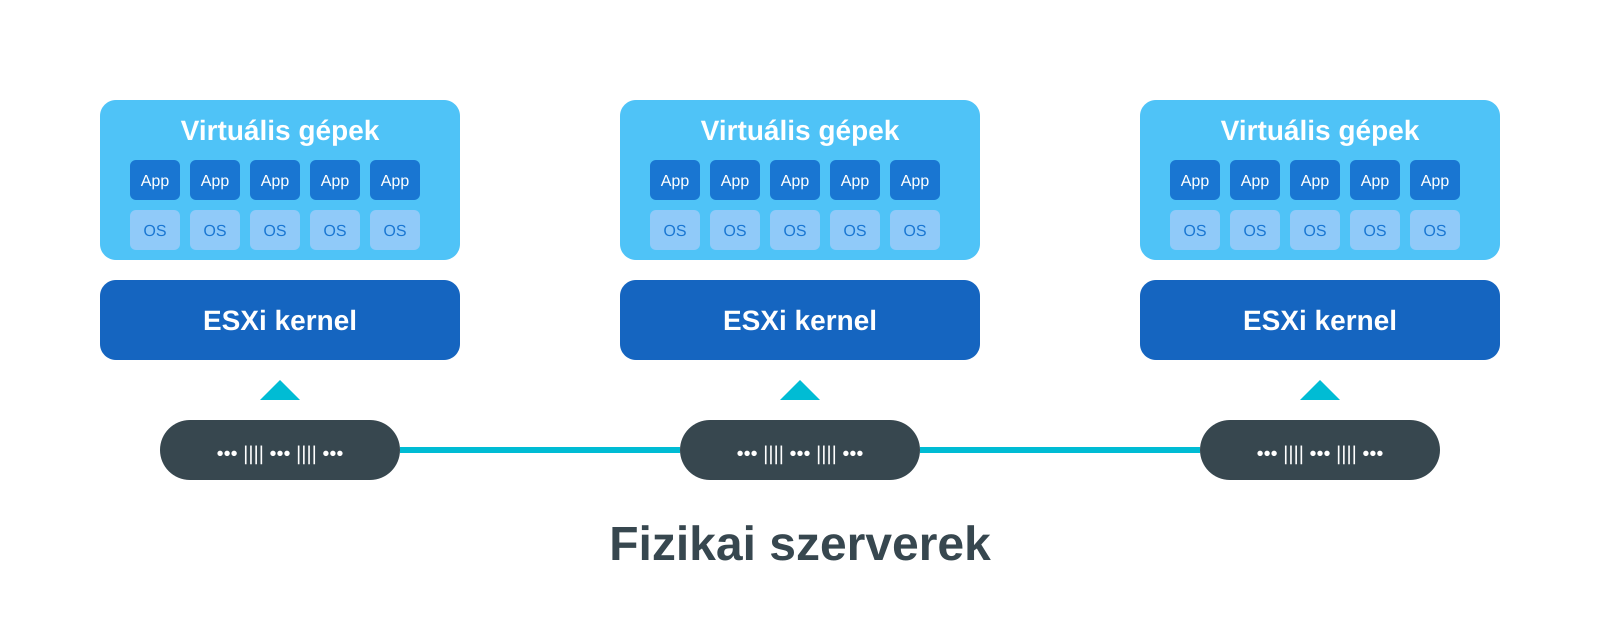
\includegraphics[scale=0.75]{images/survey/esxiexplanation.png}
        \caption{A VMWare ESXi működési elve}
        \label{esxi}
\end{figure}

Az \ref{esxi} ábrán látható a VMWare ESXi működése. A felhasználók telepíthetik
az ESXi-t a fizikai gépre, majd létrehozhatnak és kezelhetnek virtuális gépeket
a vSphere kliens segítségével. A virtuális gépek teljesen elszigetelt
környezetek, amelyek saját operációs rendszerrel rendelkeznek. Az egyes
operációs rendszereken elkülönített alkalmazások futnak.

Az ESXi operációsrendszer-független. Közel áll nagyon egy hagyományos operációs
rendszerhez, mivel saját kernellel és felhasználói felülettel rendelkezik. Ez a
komplexitás azonban nem száll át a virtualizált operációs rendszerek
rendszergazdáira. Ugyanakkor nem olyan rugalmas, mint más virtualizációs
megoldások, például a KVM vagy a Xen, mivel csak bizonyos
hardverkonfigurációkat támogat.

\subsection{KVM}

A KVM rövidítése a \textit{Kernel-based Virtual Machine}-nek, ami egy nyílt
forráskódú virtualizációs technológia, amely a Linux kernelbe van integrálva. A
KVM lehetővé teszi, hogy egy Linux rendszeren hipervizorként futva több
virtuális gép futtatható legyen egyetlen fizikai gépen.

A VMware ESXi-hez képest a KVM nyílt forráskódú. Rugalmasabb, hiszen a
felhasználók a szokásos Linux parancsokkal hozhatnak létre és kezelhetnek
virtuális gépeket. A KVM emellett pehelysúlyúbb is, mivel a meglévő Linux
kernelt használja a virtualizációs képességek biztosításához, ahelyett, hogy
külön hypervisort igényelne.

A VMware ESXi-t leginkább vállalati környezetben telepítenek, míg a KVM-et
inkább felhőkörnyezetekben használják, vagy olyan fejlesztők, akik virtuális
gépeket szeretnének futtatni saját hardverükön. A Linux hardvertámogatását
kihasználva számos hardverkonfigurációt támogat. Emellett ingyenes, ami miatt
számos tárhelyszolgáltató kínál KVM-alapú virtuális privát szervereket (VPS)
versenyképes áron. \cite{xenkvm}

Azonban mind a VMWare ESXi, mind a KVM rendelkezik korlátokkal. Elsősorban
virtuális gépek futtatására tervezték őket, amelyek erőforrás-igényesek
lehetnek, és nem feltétlenül a leghatékonyabb módja a könnyű alkalmazások vagy
microservice-ek futtatásának.\footnote{Meglepő módon még a konténerizáció is
        visszanyúl néha a virtualizációhoz, mivel néhány konténer-futtatórendszer, mint
        például a \textit{Firecracker}, biztonsági okokból KVM-et használ a konténerek
        virtuális gépen történő futtatására.} Itt jön képbe a konténerizáció.

\subsection{Konténerizáció: Docker és Docker Desktop}

\begin{figure}[!h]
        \centering
        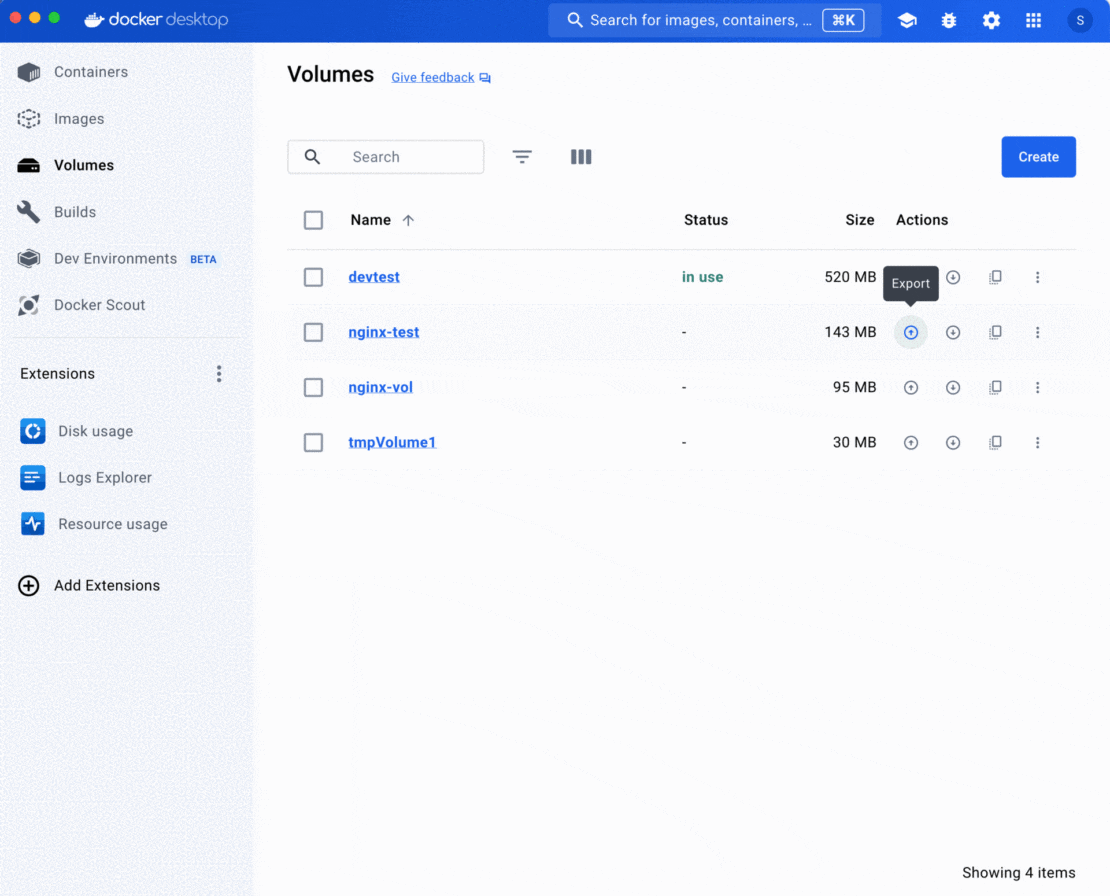
\includegraphics[scale=0.4]{images/survey/dockerdesktop.png}
        \caption{A Docker Desktop kinézete}
        \label{docker}
\end{figure}

A Docker (lásd \ref{docker}. ábra) egy részben nyílt forráskódú platform, amely
lehetővé teszi alkalmazások elkülönített konténerekben történő telepítését,
skálázását és kezelését. A Docker már a konténerizáció szinonimája. A
konténerek gyakorlatilag futó Docker image-ek, amelyek mögött egy virtuális
fájlrendszer és a hozzájuk tartozó folyamatok állnak. A Docker image-ek önálló,
hordozható környezetet biztosítanak, amelyek tartalmazzák az alkalmazást,
valamint annak minden függőségét, beleértve az operációs rendszer könyvtárait
és szükséges könyvtárakat is.

Bár a konténerek közösen használják a gazdagép operációs rendszerének kernelét
a Docker környezeten belül, biztonsági szempontból hasonló védelmet nyújtanak,
mint a hagyományos virtuális gépek \cite{containersec}. Az alkalmazás
függőségeivel egyött egyetlen egységbe zárva futnak, így minimalizálódnak az
esetleges fájlrendszerbeli konfliktusok, és biztosítható a környezet pontos
reprodukálhatósága. Mivel a konténerek mögött nem áll hagyományos operációs
rendszer, kevesebb erőforrást igényelnek, mint a hagyományos virtuális gépek,
valamint gyorsabban indíthatók. A hardvert hatékonyabban ki tudjuk használni,
és gyorsabban skálázhatjuk az alkalmazásainkat.

A Dockert és a Docker Compose-t széles körben alkalmazzuk mind a fejlesztési,
mind az éles környezetünkben. A Docker Compose segítségével definiált
szolgáltatásokat gyakran különálló projektekbe szervezzük, így ezek a rendszer
más Compose-projektjeitől függetlenül, atomi módon indíthatók, újraindíthatók
vagy leállíthatók: ezáltal a karbantartás rendkívül egyszerűvé válik.

Manapság a Docker Engine egy nyílt-forráskódú konténer-platformon alapszik, a
Moby projekten. A Moby projekt célja, hogy egy moduláris, szabadon bővíthető
alapot biztosítson konténeres rendszerek építéséhez, amelyből a Docker saját
megoldása is építkezik. Ez a projekt a Docker projektből született, amely
eredetileg egy monolitikus alkalmazás volt. A Moby projekt nyílt forráskódú, hogy a közösség felkarolásával tudják fejleszteni. \cite{ghosh2020docker} A Docker CLI-on, a Docker Swarm-on és a Docker Scout-on kívül a
Docker cég további termékei, mint például a Docker Desktop, zárt forráskódúák és
külön licenszelemeket tartalmaznak. \cite{dockerproducts}

\subsection{BSD Jails}

A FreeBSD-ből származó BSD Jail mechanizmus egy könnyű, operációs rendszer
szintű virtualizációs technológia, amely megelőzte a Dockerhez hasonló
konténerek széles körű elterjedését. A jail ugyan nem egy teljes értékű
virtuális gép, de biztonságos, elszigetelt környezeteket (``jail'') hoz létre
egyetlen FreeBSD operációs rendszeren belül. Minden jail saját hostnévvel,
IP-címmel és külön fájlrendszerfával rendelkezik, így a benne futó folyamatok
számára önálló rendszernek tűnik.

A BSD Jails a konténerizáció egyik legkorábbi formája, amely a teljes hardveres
virtualizáció többletköltségei nélkül kínál folyamat-, fájlrendszer- és
hálózati izolációt. Úttörő szerepük ellenére nem értek el olyan széles körű
elterjedést, mint a későbbi konténertechnológiák, például a Docker, amely
hatalmas népszerűségre tett szert. Ez egyrészt technikai paradoxon, mivel
Linuxon a konténerizáció gyakran több, egymástól eltérő kernelfunkció
kombinálásával valósul meg (például a cgroups az erőforrás-kezeléshez és a
namespaces az elszigeteléshez), míg a BSD Jails egy integráltabb és egységesebb
megoldást kínál magában a FreeBSD kernelben. Végül a Docker győzött a könnyű
használhatóságával, az ökoszisztémájával és - ami talán a legfontosabb - a maga
köré épített közösségével.

\subsection{Podman}

\begin{figure}[!h]
        \centering
        \includesvg[scale=1.5]{images/survey/podmanlogo.svg}
        \caption{A Podman logója}
        \label{podman}
\end{figure}

A Podman (\ref{podman}. ábra) egy nyílt forráskódú, daemon nélküli
konténerkezelő eszköz. A Dockerhez hasonlóan a Podman is lehetővé teszi a
konténerek építését, futtatását és kezelését, azonban jelentős különbséggel:
nem igényel háttérben futó daemon folyamatot mint a Docker Engine. Ez a daemon
nélküli architektúra növeli a biztonságot, mivel a konténerek közvetlenül a
felhasználó folyamataiként futnak, elkerülve a root jogosultságú daemonnal járó
potenciális kockázatokat, ami a Docker esetében a legtöbb biztonsági aggály
forrása. A daemon, mint központi vezérlőforrás is megszűnik. A Docker esetében
a rendszer teljes kompromittálódásához vezethet, ha egy támadó hozzáfér a
Docker daemonhoz. A Podman esetében nincs ilyen veszély.

A Podman kiemelkedő tulajdonsága a \textit{rootless konténerek} támogatása, ami
azt jelenti, hogy a felhasználók root jogosultság nélkül is futtathatnak
konténereket. Ez tovább javítja a biztonságot. A Podman emellett kompatibilis a
Docker CLI-val, így a Docker felhasználók könnyedén átállhatnak rá, mivel a
legtöbb parancs azonos. Támogatja a Podokat is, amelyek lehetővé teszik több
konténer egyetlen egységként történő kezelését, ami különösen hasznos a
Kubernetes-kompatibilis munkafolyamatokhoz.

A Podman azonban nem mentes a kihívásoktól. Bár úgy tervezték, hogy a Docker
helyettesítésére szolgáljon, a Docker egyes funkciói nem támogatottak teljes
mértékben a Podmanban. A Podman például nem rendelkezik teljes körű Compose
implementációval, ami nehezítheti a több konténerrel rendelkező alkalmazások
kitelepítését. Van egy kísérlet arra, hogy áthidalják ezt Podman Compose
projekttel, de ez nem olyan kiforrt, mint a Docker Compose, és a gyakorlatban
meglehetősen könnyen hibát dob. \cite{ezeobi2024investigation}

\subsection{Containerd}

A \textit{containerd} egy olyan alapvető konténer-futtató daemon, amelyre
összetettebb konténer-orchestrációs platformok építhetők. A konténerek
futtatásához és kezeléséhez az abszolút minimumkövetelményeket biztosítja, de
nem kínál magas szintű képességeket vagy felhasználóbarát felületeket a
közvetlen interakcióhoz. Parancssori interfésze, az `ctr` elsősorban fejlesztők
és rendszerintegrátorok számára készült, hogy hozzáférjenek a
\textit{containerd} alacsony szintű belső részeihez, és nem javasolt a magas
szintű felhasználók számára.

A felhasználóbarát Docker CLI és az alacsony szintű containerd közötti szakadék
áthidalására olyan projektek jelentek meg, mint a \textit{nerdctl}. A
\textit{nerdctl} célja, hogy Docker-kompatibilis CLI-t biztosítson a
\textit{containerd} számára. A Compose implementációja azonban több problémával
is küzd, többek között helytelen zárási mechanizmusokkal, a multi-Compose
projekt támogatásának hiányával és a függőségek túl agresszív kezelésével.
Például két Compose parancsot nem lehet egyszerre futtatni a \textit{nerdctl}
használatával, mivel az a teljes Compose környezetet zárolja, és megakadályozza
több Compose parancs végrehajtását, amíg az első be nem fejeződik. Ez
alkalmatlanná teszi a programot az éles környezetben való használatra.

A többszörös Compose projektek csak megoldásokon keresztül támogatottak. Ha
például két olyan Compose-projekt van, amelyet egyszerre kell futtatni, akkor
azokat meghatározott sorrendben kell futtatni, ami bonyodalmakhoz vezethet. Nem
tudja automatikusan kitalálni a Compose projektek közötti függőségeket.
Emellett a \textit{nerdctl} függőségkezelése túlságosan agresszív, ami azt
jelenti, hogy megpróbálja újraindítani egy szolgáltatás függőségeit akkor is,
ha nem szükséges az újraindítás. Ez irreleváns szolgáltatások szükségtelen
leállásához vezet.

Azt is fontos megjegyezni, hogy a széles körben népszerű konténerplatform, a
Docker a \textit{containerd}-et használja a színfalak mögött a konténer
futtatórendszereként. Régebbi Kubernetes-verziók is a \textit{containerd}-t
használták a konténerek futtatására, de az újabb verziók már a \textit{CRI-O}
konténer-futtatót használják, amely a Kubernetes számára optimalizált futtató.

\subsection{Firecracker}

\begin{figure}[!h]
        \centering
        
\includegraphics[scale=0.12]{images/survey/firecracker.png}
        \caption{A Firecracker logója}
        \label{firecracker}
\end{figure}

A Firecracker (\ref{firecracker}. ábra) a konténer ökoszisztéma legújabb tagja. A Firecracker célja, hogy a konténerek gyors indítási idejét és alacsony erőforrás-felhasználását a virtuális gépek (VM-ek) által biztosított erős elszigeteltséggel kombinálja. Ehhez a KVM ökoszisztémáját használja, amely segítségével pehelysúlyú virtuális gépeket, úgynevezett microVM-eket hoz létre, amelyek minimális többletköltséggel futtathatók egy gazdaszámítógépen.

Egyetlen fizikai gépen több száz mikroVM futhat párhuzamosan, mindegyik saját kernel-lel és minimális rendszerrel. Ezek a mikroVM-ek gyorsan, akár 125 ms alatt elindíthatók, és mindössze néhány megabájt memóriát igényelnek \cite{agache2020firecracker}. A Firecracker minimalista megközelítése révén csak a legszükségesebb eszközöket és interfészeket tartalmazza, csökkentve a támadási felületet és növelve a biztonságot. Mivel Rust nyelven íródott, a Rust memóriabiztonsági garanciáit is kihasználja, ami megelőzi a biztonsági réshez vezető gyakori programozási hibákat.

Másrészt, mivel a virtio eszközökön keresztül kommunikál, nem olyan rugalmas, mint más konténer-futtatórendszerek. A Firecracker microVM-ek nem oszthatják meg a host fájlrendszerét, ami azt jelenti, hogy minden microVM-nek saját block device-okat és fájlrendszerképet kell készítenie. Ez megnehezíti az integrációt például a Zebrafish-sel, amelynek szigorú követelményei vannak az operációs rendszer által biztosított fájlrendszer használatára, ami lehetővé teszi az erős adatkonzisztencia és az automatikus adattükrözés/mentési politika alkalmazását. A Firecracker továbbá nem tud kommunikálni a hoszt eszközökkel, ami azt jelenti, hogy a Firecracker platformon nem lehetne gyorsított gépi tanulási munkaterheket, például fényképek osztályozását futtatni, mivel a hoszt gép GPU-ját nem lehetne elérni.

\subsection{Kubernetes}

\begin{figure}[!h]
        \centering
        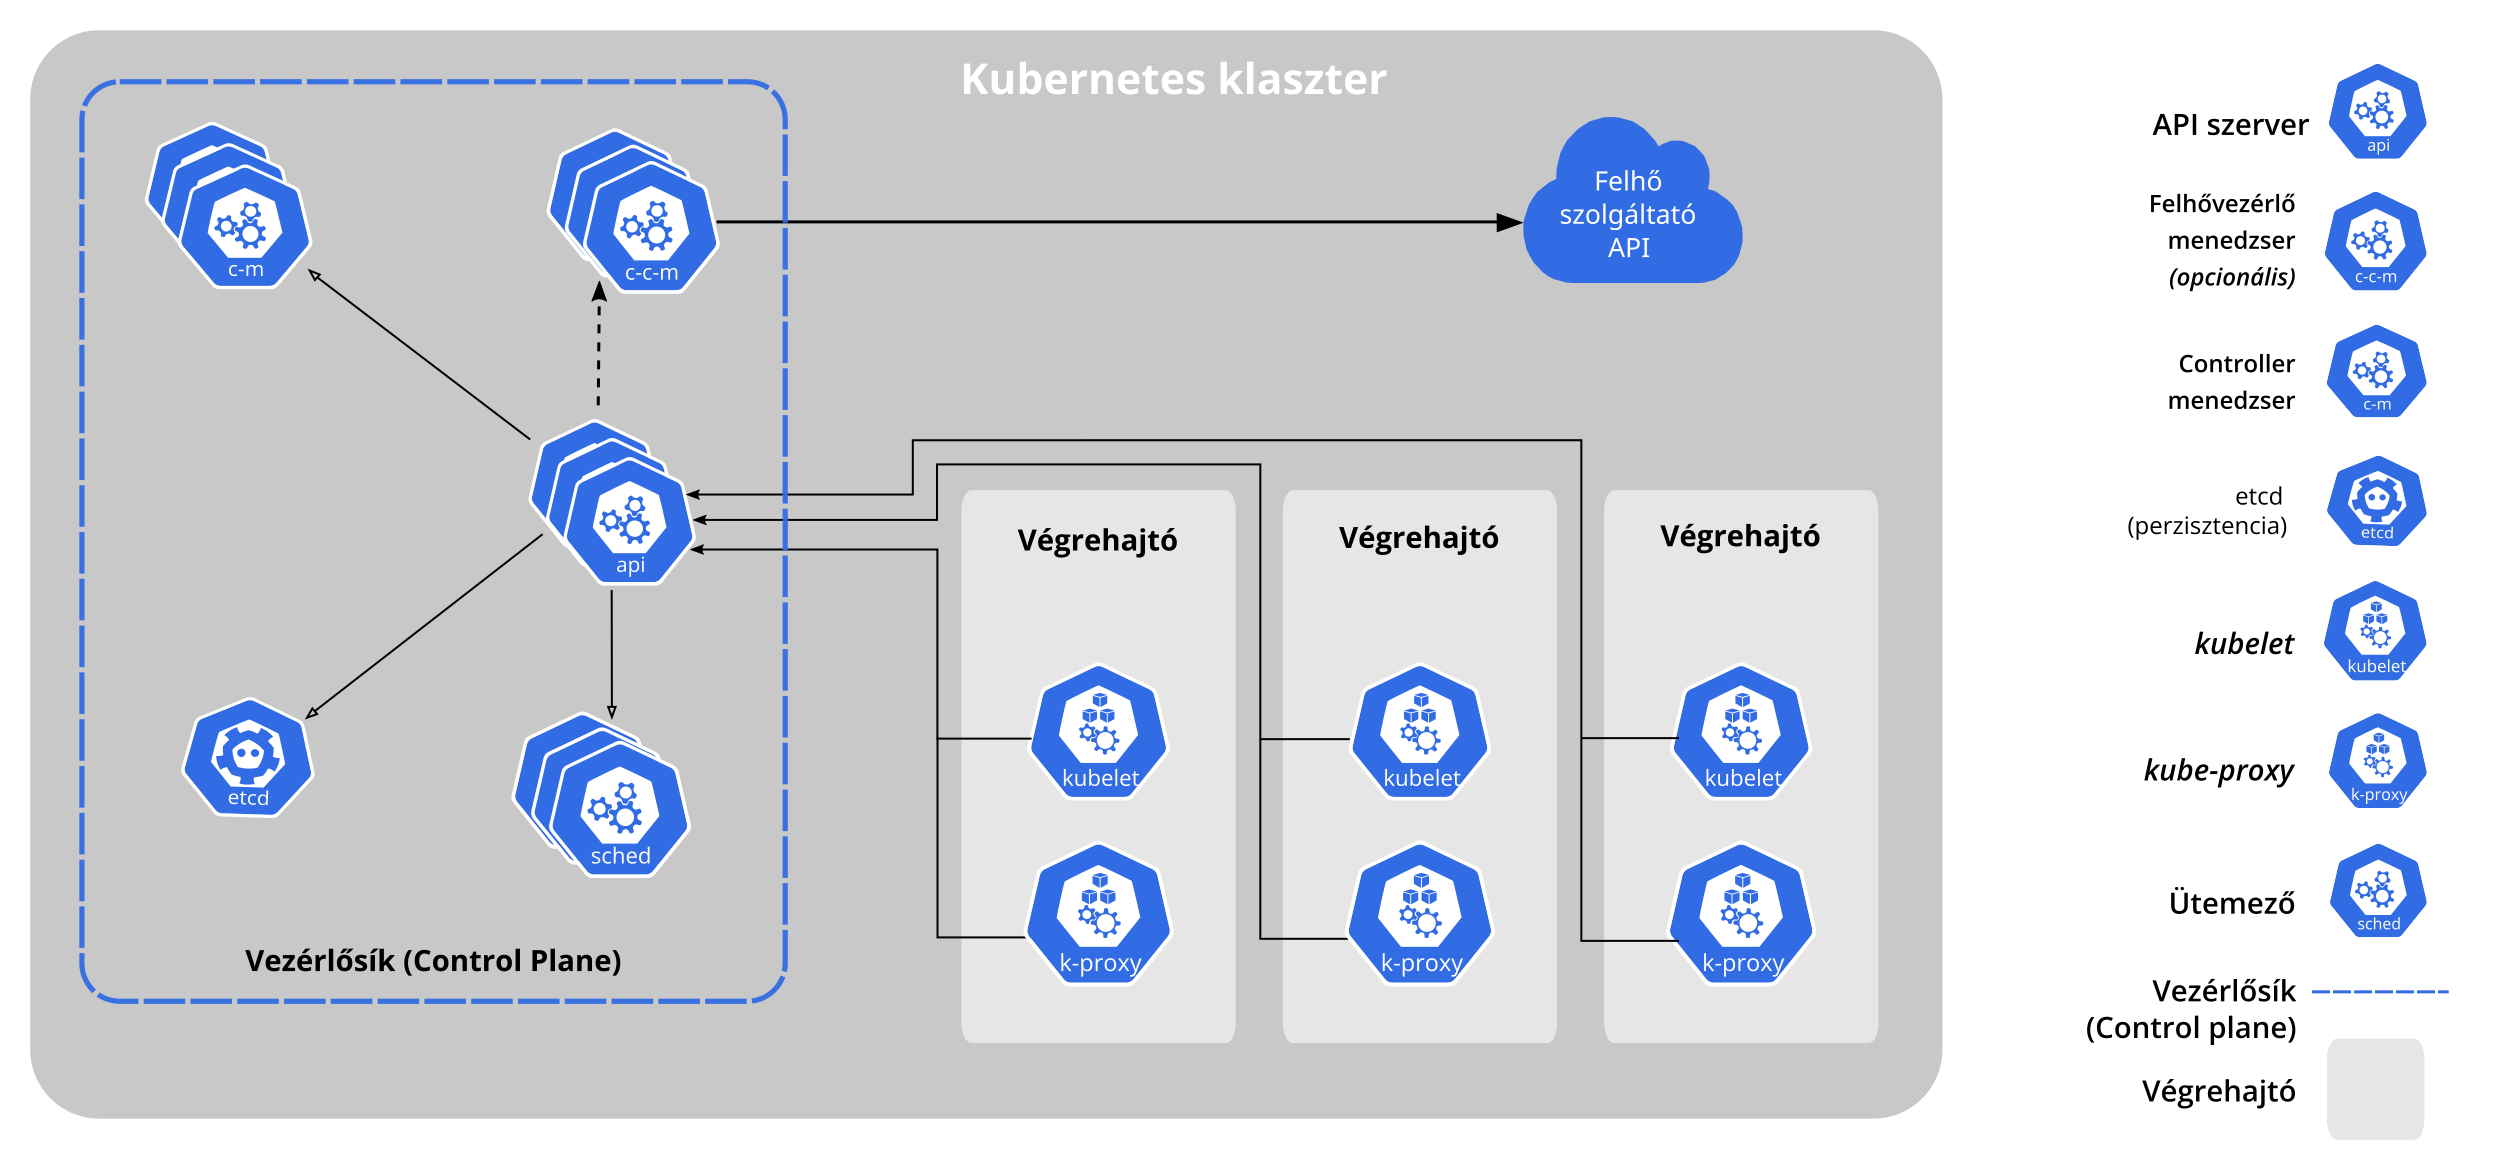
\includegraphics[scale=0.5]{images/survey/kubernetes.png}
        \caption{A Kubernetes architektúrája}
        \label{kubernetes}
\end{figure}

A Kubernetes (\ref{kubernetes}. ábra) egy nyílt forráskódú
konténer-orchestrációs platform, amely automatizálja a konténeres alkalmazások
telepítését, skálázását és kezelését. Eredetileg a Google tervezte, és a Cloud
Native Computing Foundation (CNCF) tartja karban. A Kubernetes egy
többcsomópontos platform, amelyet több fizikai vagy virtuális gépen
(csomóponton) való telepítésre terveztek. Ezáltal biztosítja a magas
rendelkezésre állást és a skálázhatóságot. Lehetővé teszi a fejlesztők számára,
hogy deklaratívan definiálják az alkalmazásaik kívánt állapotát. A Kubernetes
gondoskodik arról, hogy ez az állapot fennmaradjon: kezeli a hibákat, a
terheléselosztást és a skálázást.

A Kubernetes fő komponensei közé tartozik a \textit{master node}
(vezérlőcsomópont) és a \textit{worker node}-ok (munkavégző csomópontok). A
vezérlőcsomópont felelős a klaszter állapotának fenntartásáért, a munkavégző
csomópontok pedig a konténerek tényleges futtatásáért. A Kubernetes deklaratív
konfigurációs fájlokat használ (általában YAML formátumban), amelyekben
leírhatjuk, hogy milyen alkalmazásokat, hány példányban, milyen erőforrásokkal
szeretnénk futtatni.

A Kubernetes legfontosabb absztrakciói:
\begin{enumerate}
        \item \textbf{Pod}: A legkisebb üzemeltethető egység, amely egy vagy több konténert tartalmaz, közös hálózati és tároló erőforrásokkal.
        \item \textbf{Deployment}: Lehetővé teszi a podok deklaratív menedzselését, például a példányszám automatikus skálázását vagy frissítését.
        \item \textbf{Service}: Állandó hálózati elérési pontot biztosít a podokhoz, elrejti a podok dinamikus IP-címét, és lehetővé teszi a terheléselosztást.
        \item \textbf{ConfigMap} és \textbf{Secret}: Konfigurációs adatok és érzékeny információk (például jelszavak) kezelésére szolgálnak.
        \item \textbf{Ingress}: Külső forgalom irányítására szolgáló komponens, amely lehetővé teszi a HTTP(S) forgalom szabályozását, átirányítását a megfelelő szolgáltatásokhoz.
\end{enumerate}

A Kubernetes előnyei közé tartozik a magas rendelkezésre állás, az automatikus
skálázás, az önjavítás (például hibás podok automatikus újraindítása), valamint
a gördülő frissítések támogatása. A platform széles körben támogatott a nagy
felhőszolgáltatók (Google Cloud, AWS, Azure) által, de saját infrastruktúrán is
telepíthető.

A Kubernetes komplexitása miatt kisebb projektek esetén túl komplikált lehet,
azonban nagyvállalati környezetben, microservice-alapú architektúrák esetén
szinte iparági szabvánnyá vált. A Zebrafish fejlesztése során a Kubernetes
által kínált funkcionalitás inspirációként szolgált, azonban a cél egy
egyszerűbb, könnyebben kezelhető, fejlesztőbarát platform létrehozása volt,
amely a Compose-alapú munkafolyamatokat helyezi előtérbe, az egyszerűbb
telepítésekhez, amelyek csak egyetlen kiszolgálót igényelnek.

\section{Használt szoftverek, könyvtárak}

Ebben a fejezetben megvizsgáljuk a fejlesztés során használt szoftvereket a Zebrafish platform fejlesztéséhez.
A Zebrafish platform valóban óriások vállára épül, számos olyan szoftvert használ, amelyek közül néhányat korábban csak szabadalmaztatott platformokba integráltak, mint például a Dockerbe.

Ennek a fejezetnek a célja, hogy áttekintést adjon a felhasznált szoftverekről, valamint rövid magyarázatot arról, hogy miért ezeket a szoftvereket választottuk, és hogy hogyaan járulnak hozzá a Zebrafish működéséhez.

\subsection{A Linux kernel}

A Linux kernel számos alapvető funkciót biztosít a Zebrafish által biztosított konténerizációhoz. A Linux felelős a folyamatok elkülönítésének és erőforrásainak kezeléséért. Elsősorban a Linux névterek (namespaces) funkcióját használjuk a szükséges elszigetelés biztosítására. Másodsorban a rendszer erőforrásainak priorizálására a cgroups (control groups) funkciót használjuk.

A névterek a folyamatok elszigetelését biztosítják azáltal, hogy egy virtuális környezetet hoznak létre a folyamatok egy csoportja számára. Minden névtér úgy tűnik a benne lévő folyamatok számára, hogy egy globális rendszererőforrás saját, elszigetelt példányával rendelkeznek. A Linux kernel többféle névteret biztosít, amelyek közül a legfontosabbak, amelyeket a Zebrafish platformon használunk, a következők:
\begin{itemize}
    \item \textbf{PID névtér:} Elkülöníti a folyamatazonosítókat, ami azt jelenti, hogy a konténeren belüli folyamatoknak saját PID-készletük van. Mivel a PID 1-es folyamat az init folyamat, ő felelős a zombi folyamatok leállításáért és az árva folyamatok kezeléséért. Annak biztosítására, hogy az init folyamat ténylegesen kezelje ezeket a feladatokat, egy speciális init folyamatot (tini) használunk, amely PID 1-ként fut a konténeren belül és megvalósítja ezeket a funkciókat.
    \item \textbf{Hálózati névtér:} Elkülöníti a hálózati interfészeket, útválasztási táblákat és portokat. Minden konténer saját virtuális hálózati veremmel rendelkezik. Ezt használjuk annak biztosítására, hogy a konténerek kommunikálni tudjanak egymással és a gazdarendszerrel anélkül, hogy más konténereket zavarnának. Természetesen ehhez tartozik egy userland réteg is.
    \item \textbf{Mount névtér:} Elkülöníti a fájlrendszert. A különböző mount névterekben lévő folyamatok különböző nézetekkel rendelkeznek a fájlrendszerre. Tiszta és elszigetelt fájlrendszert biztosítunk minden konténer számára. Egy konténerben végrehajtott változtatások nem befolyásolhatják a többit.
    \item \textbf{User névtér:} Elkülöníti a felhasználói- és csoportazonosítókat, lehetővé téve, hogy egy folyamatnak egy konténeren belül egy normális, nem root jogosultságú felhasználója legyen. Ez nagyon fontos a biztonság szempontjából, mivel a konténereket ezáltal csökkentett jogosultságokkal tudjuk futatni.
\end{itemize}

A cgroups segítségével kiosztjuk a rendszer erőforrásait. Például a CPU-nak, a memóriának és az I/O-nak a prioritását és határértékeit (limitjeit) tudjuk meghatározni egy folyamatgyűjtemény számára. Ezáltal egyetlen egy konténer nem tudja monopolizálni a rendszer erőforrásait. Ha monopolizálni tudná, akkor negatív hatással lehetne a többiekre. Míg az ütemező alapból elég jó munkát végez az erőforrások elosztásában, a cgroups segítségével korlátokat és kéréseket tehetünk.

A Zebrafish platform számára alapként szolgál a Linux kernel. Rendelkezik mindazon fájlrendszer-kezeléshez és biztonsághoz szükséges kényelmi funkciókkal, amik biztosítják, hogy nem kell újra feltalálnunk a spanyol viaszt: számos fájlrendszert támogat, amelyek közül néhány erős adatkonzisztencia-garanciát biztosít; támogatja az olyan fejlett funkciókat, mint például az SMB, az NFS és az NBD, amelyek elengedhetetlenek a Zebrafish távoli fájlrendszer-képességeihez; és olyan biztonsági modellt biztosít, amely lehetővé teszi, hogy a konténereket csökkentett jogosultságokkal futtassuk, biztosítva, hogy még ha egy konténer veszélybe is kerül, a kár korlátozott legyen.

\subsection{Buildroot}

A Buildroot egy egyszerű, hatékony és könnyen használható eszköz egyedi beágyazott Linux rendszerek létrehozására keresztkompilálással (\textit{cross-compilation}). Automatizálja a teljes Linux-rendszer építésének folyamatát, beleértve a keresztkompilációs eszköztárat, a gyökérfájlrendszert, a kernelképet (\textit{kernel image}) és a bootloadert (\textit{EFI stub} vagy \texttt{syslinux}). Mivel a cél egy minimális, hatékony operációs rendszer létrehozása volt, amely \texttt{ARM64} és \texttt{x86\_64} architektúrákon egyaránt futtatható, a Buildroot-ra esett a választás.

A Zebrafish tervezése során több build rendszert is kipróbáltunk, köztük a Yocto Projectet, azonban a Buildrootra esett a választásunk az egyszerű konfigurálhatósága és a gyors ütemű közösségi fejlesztése miatt. A gyakori frissítések biztosítják, hogy mindig a legújabb szoftverekre építhetjük a Zebrafish platformot. A Kconfig-alapú konfigurációs rendszerének egyszerűsége pedig kivételesen egyszerűvé teszi az operációs rendszer képének beállítását.

A Buildroot azt is lehetővé teszi, hogy a generált lemezképekhez létrehozzunk egy \textit{software bill of materials}-t (SBOM), ami elengedhetetlen ahhoz, hogy tisztában legyünk azzal, hogy valójában milyen szoftvereket futtatunk a szervereinken. A SBOM segítségével nyomon követhetjük az összes beépített szoftverkomponenst és azok verzióit.

A projekt fejlesztése során lehetőség nyílt arra, hogy a Buildroot közösségnek változtatásokat visszaadjunk. Ez magába foglalta a javítások küldését a hivatalos levelezési listára. Értékes tapasztalat volt számomra, hiszen a Buildroot közösség, a Linux közösséghez hasonlóan, még mindig levelezőlistákon keresztül kommunikál.

A jövőre nézve a \texttt{bootc} projekt a bootolható konténer alapú operációs rendszerek érett eszközévé válhat. A \texttt{bootc} használatának további vizsgálata indokolt. Jelentős előnyöket kínálhat a rendszerfrissítések és a rendszerkezelés terén.

\subsection{Containerd és Nerdctl}

A Zebrafish platformon a konténerek futtatására a \textit{containerd} szolgáltatást használjuk. A \textit{containerd} biztosítja a konténerek életciklusának kezelését, beleértve a konténerek indítását, leállítását és monitorozását. Azonban nem biztosít lehetőséget összetettebb műveletekre, mint például Compose projektek kezelésére vagy a hálózati paraméterek beállítására.

A nerdctl egy parancssori eszköz, amely Docker-kompatibilis CLI-t biztosít a containerd számára. A nerdctl lehetővé teszi konténerek, képek és hálózatok kezelését, valamint támogatja a Compose projekteket is. A leggyakrabban használt parancsok közé tartoznak:

\begin{itemize}
        \item \texttt{nerdctl run}: Új konténer indítása egy adott imageből.
        \item \texttt{nerdctl ps}: Futtatott konténerek listázása.
        \item \texttt{nerdctl images}: Elérhető konténer image-ek listázása.
        \item \texttt{nerdctl build}: Saját image építése Dockerfile alapján.
        \item \texttt{nerdctl compose up}: Compose projekt indítása.
        \item \texttt{nerdctl compose down}: Compose projekt leállítása.
        \item \texttt{nerdctl logs}: Konténer naplóinak megtekintése.
\end{itemize}

A nerdctl CLI két legnagyobb problémája a multi-Compose projektek támogatásának hiánya, valamint az általa használt rossz zárási mechanizmus.  Még az egy-Compose-os projekteken belül is az image-ek lehúzása registryből csupán egymás után lehetséges, ami hosszú időt vehet igénybe, ha az image-ek nagyok. Ha egy image-t több helyen is használunk, akkor külön-külön lehúzza  ugyanazt. Esély sincs arra, hogy egy másodperc töredékén belül változás történt volna a feltöltött imageben.

A zárolási mechanizmus is problémás, mivel a teljes Compose környezetet zárolja, megakadályozva, hogy több Compose parancs párhuzamosan fusson. Ez a mi esetünkben jelentős korlátozást jelent, mivel gyakran kell egyszerre több Compose projektet futtatnunk.

A hálózat beállításához a nerdctl CNI integrációját használjuk, míg a Compose projektek kezelésére saját megoldást javaslunk, amely a containerd API-t használja. Ez a megoldás kompatibilis lesz a meglévő nerdctl CLI-al, így a Zebrafish CLI-al indított konténerek a nerdctl CLI-al is kezelhetők lesznek.

\subsection{CNI}

A CNI (Container Network Interface) egy szabványos interfész a konténeres hálózatok kezelésére. A Zebrafish a CNI-t használjuk a konténerek közötti hálózati kommunikáció biztosítására. A CNI különböző hálózati plugineket ad számunkra, amelyekkel beállíthatjuk a konténerek hálózati konfigurációját.

A CNI pluginok Go nyelven íródtak, és a következő pluginokat használjuk a Zebrafish-ben:
\begin{itemize}
        \item \texttt{bridge}: A legegyszerűbb hálózati plugin, amely egy Linux bridge-t hoz létre a konténerek számára. Lehetővé teszi, hogy a konténerek kommunikáljanak egymással és a gazdarendszerrel.
        \item \texttt{host-local}: Biztosítja a konténerek számára az IP-címeket. Segítségével dinamikusan osztunk ki IP-címeket a konténereknek.
        \item \texttt{firewall}: Tűzfal-szabályok alkalmazását implementálja.
        \item \texttt{portmap}: Segítségével a konténerek portjait a gazdagép portjaira le lehet leképezni (\textit{port forwarding}), így a kívülről érkező forgalom elérheti a konténereket.
        \item \texttt{tuning}: Lehetővé teszi a hálózati interfészek MTU paraméterének beállítását.
\end{itemize}

\subsection{Rust}

A Zebrafish egyes moduljainak fejlesztéséhez a Rust programozási nyelvet választottuk. A Rust egy modern, rendszerszintű programozási nyelv, amely a biztonságra és a teljesítményre összpontosít. A Rust egyik legnagyobb előnye a memóriabiztonság, amelyet a nyelv beépített tulajdonságai garantálnak, így elkerülhetők a gyakori hibák.

A Rust nyelv segítségével a fejlesztők biztosítani tudják az időbeli biztonságot és a memóriabiztonságot. A Rust fordító a fordítási időben széleskörű ellenőrzéseket végez, ami segít a lehetséges hibák korai felismerésében a fejlesztési folyamat során. Egyre nehezebb olyan kódot írni, amely nem kezeli az összes lehetséges esetet. Természetesen továbbra is lehetséges hibás kódot írni, de a fordító a hibák nagy részét már a kód futtatása előtt elkapja.

A Rust programozási nyelvben a két legfontosabb absztrakciós eszköz a \texttt{struct} és a \texttt{trait}. A \texttt{struct} típusok lehetővé teszik saját, összetett adattípusok definiálását, amelyek mezőket (fieldeket) tartalmaznak, hasonlóan más nyelvek osztályaihoz. Az \texttt{impl} blokk segítségével metódusokat rendelhetünk ezekhez a struktúrákhoz, így viselkedést adhatunk az adatokhoz.

A \texttt{trait} egyfajta interfész (szerződés), amely meghatározza, hogy egy típusnak milyen metódusokat kell implementálnia. Egy \texttt{struct} egy vagy több \texttt{trait}-et is implementálhat, így biztos megfelel annak a szerződésnek.

\subsection{Tokio}

A Zebrafishen belül a Tokio aszinkron futtatókörnyezetet használjuk a Rust nyelvben írt komponensek számára. A Tokio egy aszinkron I/O könyvtár, amely lehetővé teszi nagy teljesítményű, párhuzamosan futó alkalmazások fejlesztését. A Tokio segítségével könnyedén kezelhetjük az aszinkron műveleteket, főleg a hálózati kommunikációkat.

Más aszinkron futásidejű programokhoz képest a Tokio egy nagyon jól átgondolt és tervezett könyvtár. Gazdag funkciókészletet biztosít, beleértve az időzítőket, a csatornákat és a feladatütemezést, ami alkalmassá teszi komplex alkalmazások építésére. Úgy tapasztaltam, hogy a más nyelveken található aszinkron futásidejű futásidő, például a Python asyncio, nem olyan jól megtervezett és átgondolt, mint a Tokio.

A Tokiónak köszönhetően a Zebrafish képes több image letöltésére egyidejűleg, így a rendszer frissítése és karbantartása gyorsabbá válik, az új szolgáltatások bevezetése pedig gördülékenyebb.